\documentclass[aspectratio=1610]{beamer}
\usepackage[T1]{fontenc}
\usepackage{hardwrap}


\usetheme{wildcat}
\usetikzlibrary{shapes.geometric,arrows,positioning,fit,backgrounds}
\usepackage[backend=biber,style=authoryear]{biblatex}
\addbibresource{references.bib}

\title{Leveraging Nonlinear Systems Equation for Efficient Spam Email Detection}
\author{Group A}


\titlegraphic{
\includegraphics[scale=0.25]{680558}}

\tikzstyle{box} = [rectangle, draw, minimum width=2cm, minimum height=0.8cm, text centered, font=\footnotesize]
\tikzstyle{dashedbox} = [rectangle, draw, dashed, minimum width=3cm, minimum height=1.5cm, font=\footnotesize]
\tikzstyle{arrow} = [thick,->,>=stealth]


\begin{document}

%title page
\begin{frame}
\titlepage
\end{frame}

%slides 1 Group member
\begin{frame}{Group Members}
    \begin{center}
        \begin{tabular}{|c|l|}
            \hline
            \textbf{Matrix Number} & \textbf{Name} \\
            \hline
            S2191553 & Yerong Liu \\
            \hline
            U2100875 & HAFIZ AIMAN BIN SHAMSUL BAHARI \\
            \hline
            S2148250 & SOO WEE LIM \\
            \hline
            U2101770 & MUHAMMAD AIDIL SHAZWAN BIN MARZUKHI \\
            \hline
            S2190329 & Yulun Deng \\
            \hline
            S2109049 & SUMAIYA MUNTAREEN BILLAH \\
            \hline
        \end{tabular}
    \end{center}
\end{frame}






%slides 3 Introduction Section
\begin{frame}{Introduction}
    \frametitle{Introduction}
    \setlength{\baselineskip}{1.5em}
    Email remains a cornerstone of communication in the digital age, but its widespread use has led to the proliferation of spam emails, ranging from simple advertisements to malicious phishing and malware attempts. Traditional detection methods often fall short in addressing the complexity and adaptability of modern spam strategies. To tackle this challenge, integrating nonlinear systems equations into the \textbf{Backpropagation} process of machine learning models offers a promising solution. Nonlinear systems excel at capturing intricate patterns within data, enabling neural networks to better differentiate legitimate emails from spam while adapting to evolving threats. This approach enhances both detection accuracy and computational efficiency, providing a robust framework for large-scale email filtering.

\end{frame}

%objectives Section
\begin{frame}{objectives}
    \frametitle{objectives}
    \begin{itemize}
        \item \textbf{Reducing Data Noise: }By filtering out spam, we can ensure that important communications are not lost among irrelevant messages, improving the efficiency of email usage.
        \item\textbf{Enhance Spam Detection Efficiency: }Incorporate nonlinear system equations into the backpropagation process and loss function calculations of machine learning models to improve the model's ability to efficiently identify and filter spam emails, even as spam strategies evolve.
        \item\textbf{Improve User Experience and System Adaptability: } Optimize the model to maintain computational efficiency while adapting to changing spam patterns, ensuring a seamless, responsive email filtering system that enhances the overall user experience.
    \end{itemize}
    
\end{frame}

%Problem statement Section
\begin{frame}{Problem statement and objectives}
    \frametitle{Problem statement and objectives}
    To  detect the spam email to mitigate the security risks, reduce resource wastage, productivity loss and trust issues. 
    
    
\end{frame}

%flow chart section
\begin{frame}{Flow Chart}
    \frametitle{Basic Flow Chart (Example)}
    \begin{figure}
        \centering
        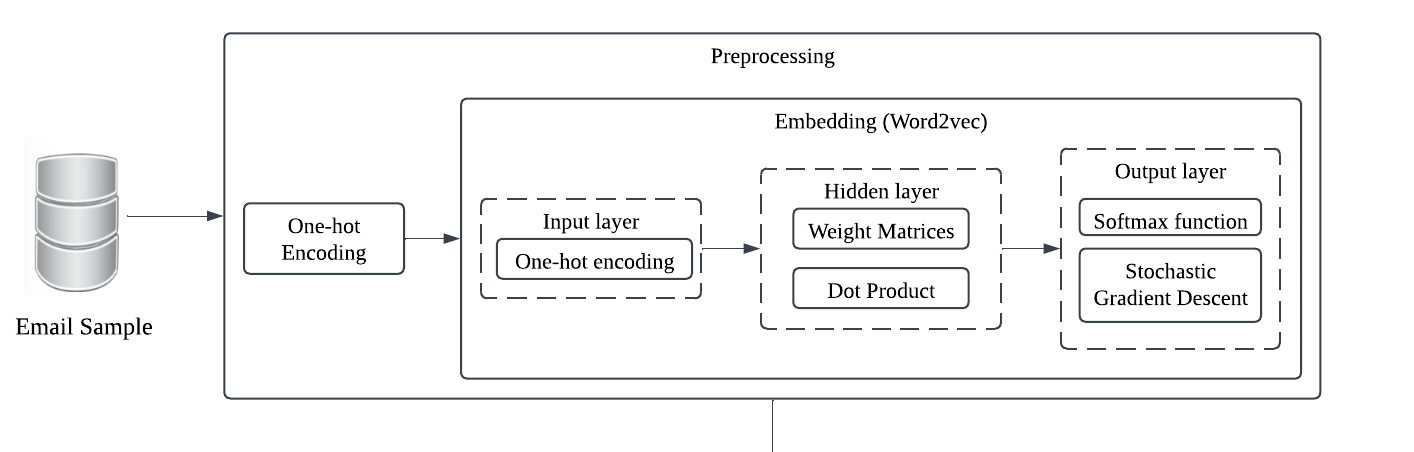
\includegraphics[width = 1.1\linewidth]{NA (1)[2]}
        \label{fig:figure}
    \end{figure}
    
\end{frame}

\begin{frame}{Flow Chart}
    \frametitle{Basic Flow Chart (Example)}
        \begin{figure}
        \centering
        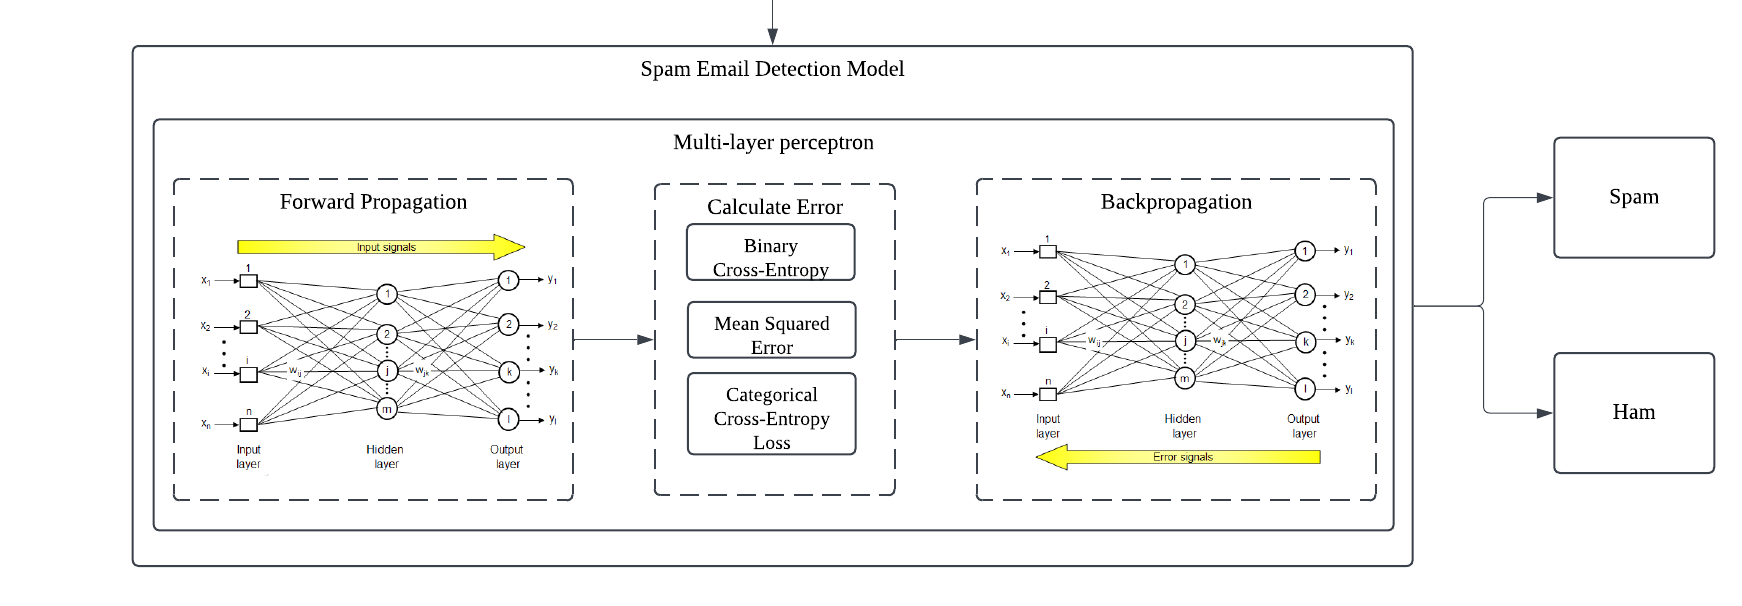
\includegraphics[width=1.1\linewidth]{D:/NA/NA (1)[1]}
        \caption{Detection Model}
        \label{fig:enter-label}
    \end{figure}
      
    
\end{frame}

\begin{frame}{Methodology}
    \frametitle{Methodology}


\end{frame}


%Conclusion section
\begin{frame}{Conclusion}
    \frametitle{Conclusion}
    
\end{frame}

\section{Thank You}








\end{document}